\documentclass[12pt]{article}
\usepackage[margin=2cm]{geometry}
\usepackage{cite}
\usepackage{float}
\usepackage{graphicx}
\usepackage[caption=false]{subfig}
  \DeclareGraphicsExtensions{.png}
\usepackage{amsmath}
\usepackage{amsfonts}
\usepackage{url}
\usepackage[edges]{forest}
\usepackage{tikz}
\usetikzlibrary{shapes,shapes.gates.logic.US,arrows,arrows.meta,chains,calc}
\tikzset{
  -|-/.style={
    to path={
      (\tikztostart) -| ($(\tikztostart)!#1!(\tikztotarget)$) |- (\tikztotarget)
      \tikztonodes
    }
  },
  -|-/.default=0.5,
  |-|/.style={
    to path={
      (\tikztostart) |- ($(\tikztostart)!#1!(\tikztotarget)$) -| (\tikztotarget)
      \tikztonodes
    }
  },
  |-|/.default=0.5,
}
\usepackage{tikz-timing}
\usetikztiminglibrary[new={char=Q,reset char=R}]{counters}
\usepackage{bm,times}
\usepackage{pgfgantt}
\usepackage{indentfirst}
\usepackage{array}
\usepackage{setspace}

\begin{document}
%\setstretch{1.0}
\begin{titlepage}
  { \Large
    Imperial College London\\[17pt]
    Department of Electrical and Electronic Engineering\\[17pt]
    Final Year Project Report \textcolor{red}{[DRAFT]}
  }

  \rule{\columnwidth}{3pt}
  \vfill
  \centering
  \includegraphics[width=0.7\columnwidth]{img/1.jpg}
  \vfill

  \begin{table}[h]
  \def\arraystretch{1.8}
    \begin{tabular}{p{40mm}p{\dimexpr\columnwidth-40mm}}
      Project Title: & \textbf{An Extensible Framework for \newline At-speed Evaluation of Arithmetic Hardware} \\
      Student:       & \textbf{Zifan Wang} \\
      CID:           & \textbf{01077639} \\
      Course:        & \textbf{EEE4} \\
      Project Supervisor: & \textbf{Dr. James J. Davis} \\
      Second Marker: & \textbf{Dr. Christos Bouganis}
    \end{tabular}
  \end{table}
\end{titlepage}

\newpage
\vspace*{6cm}
\newenvironment{acknowledgements}
  {\renewcommand{\abstractname}{Acknowledgements}\begin{abstract}}
  {\end{abstract}}
\begin{acknowledgements}
  Dr. James J. Davis for guidance

  \textcolor{red}{Should this be in references or here?}
  Junjie Lu for providing designs used during testing
  
  \textcolor{red}{Maybe the testing volunteer as well?}
\end{acknowledgements}

\newpage
\vspace*{6cm}
% This project concerns the research and design of a driving behaviour model that could identify the user from its inputs and predict his next actions for a small interval of time in the future.
% The main emphasis of this project is on implementing the necessary tools for capturing and processing the data in order to be appropriate for machine learning techniques. Using a virtual simulator, multiple users were recorded, while driving several laps of different tracks.
% The user’s actions recorded were the angles turned on the steering wheel, strength applied to the gas and brake pedals, the gears involved and speed of the car.
% By experimenting with numerous algorithms and approaching different models, it was observed that driving is a sequential model that depends on the previous and current driver’s actions, the car’s response and the environment.
% Random Forests, Decision trees and Hidden Markov model algorithms have been used with both independent windows of data and sequences of data for predicting, with high accuracy, the identity of the driver.
% Feature extraction as well as feature selection algorithms were introduced to increase the performance of the classifiers.
% Experiments concerning sequences of feature vectors resulted on more accurate identification of the users.

\begin{abstract}
This project concerns the research and design of a driving behaviour model that could identify the user from its inputs and predict his next actions for a small interval of time in the future.
The main emphasis of this project is on implementing the necessary tools for capturing and processing the data in order to be appropriate for machine learning techniques. Using a virtual simulator, multiple users were recorded, while driving several laps of different tracks.
The user’s actions recorded were the angles turned on the steering wheel, strength applied to the gas and brake pedals, the gears involved and speed of the car.
By experimenting with numerous algorithms and approaching different models, it was observed that driving is a sequential model that depends on the previous and current driver’s actions, the car’s response and the environment.
Random Forests, Decision trees and Hidden Markov model algorithms have been used with both independent windows of data and sequences of data for predicting, with high accuracy, the identity of the driver.
Feature extraction as well as feature selection algorithms were introduced to increase the performance of the classifiers.
Experiments concerning sequences of feature vectors resulted on more accurate identification of the users.
\end{abstract}

\newpage

\setcounter{tocdepth}{2}
\tableofcontents

\newpage
%\setstretch{1.5}

\chapter{Introduction}

With the right number representation system, it is possible to perform arithmetic operations MSD first.
Consequently, these online arithmetic operators are attractive for hardware implementation in both serial and parallel forms.
When computing digits serially, they can be chained such that subsequent operations begin before the preceding ones complete.
Parallel implementations tend to be most sensitive to failure in their LSDs, making them more friendly to overclocking than their LSD first counterparts, for which the opposite is true.
In the past, online operators have typically been implemented in binary.
Although Radix-2 modules are the simplest to design and have the shortest cycle time per digit, they have the highest online delay and require the largest number of cycles to complete calculations~\cite{Tenca1}.
As such, the choice of binary is not absolute.

The initial goal of this project is thus to build a testbench that can investigate the operators' suitability for FPGA implementation and examine the resultant tradeoffs between performance, area and power.
However, after some time researching and working on the project, we realised that the testbench can be extended to a more general testing framework with some effort.
This makes the project much more meaningful in the long term, as researchers working on other arithmetic units can also utilise this testbench after some configuration.
The focus of the project thus shifted to delivering a customisable and extensible verification system while retaining the at-speed testing capabilities needed for the starting goal.

In this report, we will first discuss the motivations of investigating high-radix online arithmetic hardware on FPGAs in chapter 1.
Following which the design of the evaluation framework will be put forth in chapter 4, and the design process of each individual module will be examined in detail in chapter 5 and 6.
After determining the preferred designs, we will present how each module was built on the FPGA development board in chapter 7, 8 and 9.
With the implementation complete, the framework itself will be evaluated to see if it fulfilled its purposes in chapter 10.
The results of this test will be subsequently analysed in chapter 11, and the report will conclude in chapter 12 before the proposing a few ideas for further improvement of the product in chapter 13.


\chapter{Background}

\textcolor{red}{Need new motivation after generalising project?}


\newpage
\section{Project Specification}

\subsection{Project Organisation}
This project is a part of a larger project investigating the effect of using high-radix number representation with online arithmetic operators.
The overarching aim involves implementing such a system on an FPGA and quantifying its performance improvements.
This is achieved through two individual projects, vertically split from the enveloping project.
One shall design the arithmetic operator modules, while the other shall design a system from the top-level to test and evaluate these operators.
This project deals with the system-level issues.

As this project progresses in parallel with the designing of the operator modules, it is necessary to decouple the two projects so that, being individual projects, they can be evaluated individually.
The success of one project should not be restricted by the status of the other.
To this end, the goal of the system-level design is more focussed on its functionalities and robustness.
This relationship and its effect on the evaluation will be examined further in the evaluation chapter of this report.

To ensure the two products will work together once they are both complete, a common interface is agreed upon.
The interface will be done using Qsys.
The unit-level project will build different operators, which can have varying arithmetic functions and designs.
These can be packaged into individual Qsys modules, as adders, multipliers, or dividers.
Alternatively they can also be delivered as a single module taking two operands and an instruction that is one of the four basic arithmetic operations.
These will then become the DUTs of the testbench.

\subsection{Deliverables}
At the end of the project, the system should be able to perform the following:
\begin{enumerate}
  \item Connect to the arithmetic modules as its input;
  \item Generate and run tests on these modules;
  \item Vary the frequency of the FPGA;
  \item Evaluate its performance.
\end{enumerate}


\newpage
\section{System-level Design}

\subsection{Testbench Architecture}
The design of the verification system is the major engineering challenge of this project.
While there have been many similar performance analyses done on hybrid SoCs before, each of them used their own, usually ad hoc, testbench design~\cite{Shi1}~\cite{Li1}.
As such, most testbench are not designed to be scalable or portable, serving only what they are built for.
In this project, I shall use a generic structure inspired by that of an agent in Universal Verification Methodology (UVM).

Before UVM, integrated circuit designs were verified with methodologies developed independently by stimulator vendors such as Cadence, Mentor Graphics, and Synopsys.
In an effort to unify for greater efficiency, the standards organisation of the Electronic Design Automation (EDA) industry, Accellera, established UVM with support from multiple vendors.
It provided a common structure for verification, with class libraries that made building and running a testbench a significantly smoother experience.
The agent is a container in UVM that emulates and verifies DUTs~\cite{Accellera1}.
While this project is in no position to achieve what UVM has done, I do hope that this testbench would have an easily modifiable structure that will make the process of testing similar future designs slightly simpler.

\begin{figure}[H]
  \centering
  \input{interim/block}
  \caption{Block diagram of the proposed testbench}
  \label{Block}
\end{figure}

Configuration is first done from software running on the HPS, which sends the test specifications to the randomiser.
The randomiser will provide a stream of random data that will be converted to meaningful test inputs by the driver.
The test output will be watched by the monitor, reporting any interesting event to the scoreboard, which keeps track of them.
The scoreboard feeds the information back to the software on demand.
The interface is used to decouple the control logic from the DUT, allowing the frequency of the DUT to be finely controlled.

\subsection{User Interface}


\chapter{Hardware Design}

\section{Providing Test Data}
In order for the driver to stress the DUT, the verification system must perform at a much higher frequency than the expected frequency of the DUT.
Assuming the DUT is to run at 300MHz, to fully explore the effect of overclocking, the testbench must be able to run at double the frequency.
This gives an ambitious target frequency of 800MHz.
Assuming a data width of 32-bit, the target data transfer rate is then estimated to be 25.6Gbps.
With this rough estimate, we can start considering different design options.

\subsection{HPS-FPGA Bridge}
As the testing is to be controlled by the HPS, the HPS-FPGA bridge will be the immediate bottleneck if the test data is to flow from HPS to FPGA.
While the HPS can easily generate test data with a piece of software, there is a large amount of overhead as data crosses from one architecture to another.
This overhead exists in the form of both decreased bandwidth and increased delay.
Thus, it is not be sensible for the HPS to send out data during runtime.

\subsection{Off-chip DDR SDRAM}
Another thought may be to first populate the off-chip DDR SDRAM on the FPGA side, then feed that data to the DUT during test.
This is already much faster than passing the data directly from HPS.
The 1GB, 32-bit wide DDR3 on the FPGA side is rated at 400MHz.
With double rate transfer, this gives a maximum transfer rate of 25.6Gbps.

Although using the off-chip RAM may theoretically achieve the targets, it still has its disadvantages.
Firstly, the process of filling up the memory takes time.
Thus, the testing would be broken up into bursts, with time in between for checking results and filling in new data.
The complexity of the SDRAM interface also requires an SDRAM controller to be used to manage SDRAM refresh cycles, address multiplexing and interface timing.
These all add up to significant access latency.
While it could be overcome with burst and piplined accesses, it would further complicate the SDRAM controller.
A controller is provided by Intel~\cite{Altera3}, but it would consume a non-negligible amount of the limited FPGA resources while adding unnecessary complexities to the design.
Customising or building a new SDRAM controller to fit this project is possible, but needlessly time-consuming.

\subsection{On-chip Memory}
The on-chip memory is much faster and simpler to use.
In comparison, this memory is implemented on the FPGA itself, and thus needs no external connections for accesses.
It has higher throughput and lower latency than the SDRAM.
The memory transactions can also be piplined, giving one transaction per clock cycle.
With an on-chip FIFO accessed in dual-port mode, the write operations at one end and the read operations at the other end can happen simultaneously.
This feature is useful as tests are prepared and fed into the DUT, or when test results are collected and fed to the monitor.

On-chip memory is not without its drawbacks.
It is volatile like SDRAM and very limited in capacity.
SDRAMs can have store about 1GB, while on-chip memory could only hold a few MB~\cite{Altera2}.
Volatility is not exactly of concern in this project, but its small capacity means not much test data can be held before it needs more fed in.

\subsection{Distributed RAM / Registers}
On-chip memory has a minimum latency of 1 clock cycle as the R/W access gets processed.
If a even faster memory is desired, we can use LUTs or registers to store them.
This option would eliminate the latency but takes up much more FPGA resources.
The capacity is even more limited as LUTs are usually used for logic.
There will be a significant amount of data generated during testing, and the testbench should be as lightweight as possible to allow flexibility in the DUTs.
As such, distributed RAM will not be used in this project for data transfer.
Registers will still be used as they are essential for many other purposes.

\subsection{Real Time Data Generation}
As seen from the analysis, the best design option here should be able to exploit the benefits of on-chip memory, and circumvent the drawback of buffering testing data generated from the HPS.
Generating testing data at runtime, on the FPGA will be such a method.
As arithmetic operators have a vast set of valid inputs, it is necessary to have cost-effective test generation.

A good choice here is to use random testing.
With relatively low effort, random testing can provide significant coverage and discover relatively subtle errors~\cite{Duran1}.
The main drawback of random testing is the possible lack of coverage for corner cases, for which the usual solution is to provide handwritten tests to complement it.
However, as the main goal of this testbench is gauging the performance of the module, and not necessarily verifying the correctness of the module, having uncovered testing holes is acceptable during stress testing.
As the project progress, special tests could be written and run separately with a relaxed timing restriction to cover the holes.
It should be noted that certain corner cases may represent critical paths in the design.
To combat this, the testbench provides the option to run handwritten inputs alongside random tests.

\section{Randomiser}

LFSRs are a reliable way of generating pseudorandom numbers quickly with low cost~\cite{Hazwani1}.
Fulfilling the design requirements, they will thus form the starting point of data generation.
While it is possible for data generated to be invalid as inputs to the DUT, this should not be the case for most arithmetic units.
Even if this is the case, they can be dealt by the filter in the driver.
On the flip side, LFSRs go through every single possible value except for one before repeating itself in a loop, so it is more efficient than a purely random data set.
The one impossible value can be covered manually, and knowing that there is an impossible value from the randomiser can be turned into a design advantage later on when we make the driver.

Following this approach, the software would only need to configure the generation at the beginning, and test data no longer needs to pass through the HPS-FPGA bridge.
Thus, the testbench can provide fast and constant data to stress the DUT.

\subsection{LFSR Configurations}

While LFSRs are simple hardware modules, there are still a few design options we should explore before implementing them.
To compare, we can examine an 8-bit LFSR with taps on bit [7,5,4,3].

In a Fibonacci LFSR, the taps are pulled and fed into a cascade of XOR gates.
The output of the final XOR gate is then the lowest bit of the next random number.
The higher bits are obtained by one left bitwise shift.

\begin{figure}[H]
  \centering
  \input{illu/fibonacci}
  \caption{Fibonacci Configuration}
  \label{FibLFSR}
\end{figure}

In a Galois LFSR, the new bits in the taps are obtained by a XOR operation between the lowest bit and the bit on the left of each tap.
The highest bit is simply the previous lowest bit, and all other bits are obtained by one right bitwise shift.

\begin{figure}[H]
  \centering
  \input{illu/galois}
  \caption{Galois Configuration}
  \label{GalLFSR}
\end{figure}

Other LFSR configurations such as Xorshift~\cite{Marsaglia1} exists, but they are mostly designed and optimised as pieces of software, thus being less appropriate for this design.

By examining the two configurations, we can see that Fibonacci LFSRs have to XOR multiple bits together through a cascade of 2 input XOR gates, or a single XOR gate with multiple inputs.
On the other hand, Galois LFSRs have multiple XOR gates working independently.
On an FPGA, the cascade of gates is usually implemented with a LUT, so while limiting LUT input to 2 might have some minor improvements, this increased delay of the Fibonacci configuration should not be obvious.

In terms of implementation, Fibonnaci LFSRs are slightly easier to code if width configurability is desired.
However, building a configurable Galois LFSR is only slightly more complex.

As such, we need to take a step back and examine the overall structure of the randomiser to help us make this decision.

\subsection{Randomiser Structure}

A horizontally structured randomiser uses all bits in the LFSR as output.

\begin{figure}[H]
  \centering
  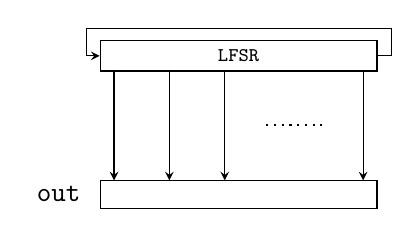
\begin{tikzpicture}
  [
    x=1em, y=1em
  ]
  \node at (-1.5, 0) {\texttt{out}};
  \node [draw,minimum height=1em, minimum width=10em] at (5, 0) (o) {};
  \node [draw,minimum height=1em, minimum width=10em] at (5, 5) (1) {\scriptsize \texttt{LFSR}};
  \draw [->, >=stealth] (1.east) -| ++(0.5, 1) -- ++(-11, 0) |- (1.west);
  \foreach \pos [count=\idx] in {0.5, 2.5, 4.5, 9.5}{
    \draw [->, >=stealth] (\pos, 4.5) -- (\pos, 0.5);
  }
  \draw [dotted, thick] (6, 2.5) -- (8, 2.5);

\end{tikzpicture}
  \caption{Horizontal Structure}
  \label{HoriLFSR}
\end{figure}

A vertically structured randomiser uses multiple LFSRs, and combines one bit from each LFSR for its output.

\begin{figure}[H]
  \centering
  \input{illu/vertlfsr}
  \caption{Vertical Structure}
  \label{VertLFSR}
\end{figure}

The horizontal option is easy to construct, but changing the width of the output value requires writing another wider LFSR since the tap positions would change.
The vertical options is much more scalable as more or less LFSR can be instantiated depending on the required output width.
As the widths of individual LFSRs are not related to the width of the output, a series cheap, 2-tap LFSRs can be used for it, making the earlier point of additional delay for Fibonacci LFSRs a non-issue.

However, the vertical structure is not without downsides.
Each LFSR needs a unique seed for its initialisation, making increasing the width not completely automatic unless we also build something that generates these seeds.
More importantly, the structure reduces the test efficiency introduced by LFSRs.
A single LFSR will go through every non-zero value before repeating itself, the vertically arranged randomiser will have early repeats.

If we allow early repeats, then the horizontal structure can be easily scaled.
This is achieved by building a long LFSR and taking a trucated version of the output value when fewer bits are required for the tests.

As such, there is no real advantage of using the vertical structure.
With truncation providing the configurability in the horizontal structure, the slight advantage of the Fibonacci LFSRs in its ease to write is nullified.
Having the slight advantage in terms of speed for Galois LFSRs, they will be chosen as the randomiser design in this project.

\section{Driver}

The driver should have two main types operation when feeding data into the DUT.
One is the stress testing mode, where the driver tries to pushes a new piece of data into the DUT at every clock tick.
The alternative is a slow manual mode, where the driver reads from the HPS-FPGA bridge and changes its output to the DUT whenever a new test point is specified by the software.
The stress testing mode will expose the DUT to as much random test points as possible in the test duration.
The manual mode is used when the user has a special interest in a limited list of inputs.

\subsection{Stress Testing Mode}
The vanilla way of providing data to the DUT is to for the driver to simply instantiate the same number of randomisers as the number of inputs of the DUT.
Then the randomisers' outputs can be directly connected to the inputs of the DUT.

While this fast and cheap method fulfils most of the requirements of the testbench, it suffers from a few issues.
One, there is no user control for the test data.
If we consider the LFSR pseudo-random number sequence to be unpredictable, then the only thing the user can do will be forcing the LFSRs to initialise with same of different seeds and therefore the DUT will receive identical or different inputs.
However, this level of customisation mostly meaningless.

\subsection{Input Filtering}
To introduce some level of non-trivial user control in the test data without losing speed, a filtering system is included in the driver design.
The filtering system needs to be fast since this is still a stress test, yet it should provide as much utility as possible to the users.

A possible design here is to allow the user to specify a maximum and a minimum bound to the value of the input data.
Each output from the randomiser is compared to these values and either sent forward if they passed or replaced if they failed the comparisons.
If a higher level of control is desired, there can also be a list of invalid inputs within the bounds of validity.
However, the latency can get high if the list is long and the comparisons can get slow if the high or low bound is irregular in its binary form.
The replacement system can also get complex if the bounds are strict.

A better alternative to achieve this is a bit manipulation system.
The user can force individual bits in the data to be cleared or set.
This is less flexible than the first design, but with some tricks the user is still able to perform a great level of input control.
Having only odd or even test inputs will be trivial under this system.
To set maximums or minimums for the test data, the user can simply set or clear the higher bits.
Certainly this imposes a strong preference to arithmetic units with regular binary representations, but most interesting designs for high-radix arithmetic units, including the ones that spawned this project, use a radix that is a power of 2.
As such, the binary manipulation system will always be helpful for the user to filter out uninteresting test points or to focus in on more meaningful ones.

\subsection{Manual Input Mode}

As discussed in the randomiser section, random testing is surprisingly useful, but they do have their limits.
If the user has a list of inputs that will trigger key logic paths in their design, they should be able to investigate them under this framework.
This would serve as a good compliment to the random testing.
The manual input mode is designed for this scenario.
In this mode, the user first provides a list of numbers when configuring the test in software, and enable the manual input mode.
Then, the test software will read through this list and write them to a set of memory locations on the HPS-FPGA bridge.
A simple transfer protocol will be used for the driver to read these locations and then forward them to the DUT.
Due to the limitations of the bridge, the DUT cannot be fully saturated with these data.
As such, each manual test input will be repeatedly sent to the DUT before the next one becomes available.

\subsection{Synchronised Monitor Inputs}
In addition to controlling what gets sent to the DUT, the driver has the responsibility to ensure that the monitor receives the test output from the DUT and the test inputs from the driver at the same time.
After going through the filtering logic, the stream of test input will not only be sent to the DUT, but also sent to a shift register before reaching the monitor.
The shift register will provide the delay required for the DUT to finish its operations.
Since the number of cycle delay from input to output should be consistent and known by the user, the length of this delay can be configured before compiling the testbench.


\section{Monitor}

Another concern in the system design is of the different clock domains that must exist on the FPGA.
Since it is not sensible to require the reference design to run as fast as the DUT, there needs to be two clock domains in the system.
The initial idea is to have one domain surrounds the DUT and another that supports the rest of the control logic around the DUT.
These clock frequencies can be generated with PLLs, which are provided as IP Cores in the Quartus software~\cite{Altera4}.
A clock tree will distribute them to the individual modules.
Data crossing clock domains will be fed through FIFOs to prevent loss.

The proposed structure will have the bulk of the control logic running in a separate clock domain to the DUT.
Only an interface with FIFOs will be running in synchronicity with the DUT.
Therefore, the test controls can run at a slower frequency without bottlenecking the system, allowing the DUT to be stressed further.
The problem now is to ensure the monitor can handle the stream of DUT output coming in at a higher frequency that it is running at.
As the monitor needs to calculate the correct data before it can check if the DUT output is correct, it cannot keep up with the speed of the DUT.
This report consider three alternatives.

\subsection{Partial Monitors}
A lightweight idea is to implement a parity checker instead of a full model inside the monitors.
For example, to check an adder, the monitor can just check if the final bit with a LUT acting as a XOR gate.

Although this is reasonably fast, it cannot be extended once the DUT is faster than a parity calculation followed by a comparison.
More critically, it provides no additional information once the DUT fails, and it has a 50\% rate of ignoring an error.
If this is to be solved by increasing the number of bits checked, the problem returns back to its initial state.
Thus this method will not be experimented.

\subsection{Lazy Monitors}

\begin{figure}[H]
  \centering
  \includegraphics[width=12cm]{img/LazMon}
  \caption{Structure of a Lazy Monitor}
  \label{LazMon}
\end{figure}

An more scalable alternative is to have the monitor only check a selection of data sets.
For example, if the monitor is programmed to check every third test point, statistically it will make little difference to the final result.
In case the DUT is aware of this and only produce correct outputs on every third operation, this process can be randomised too.

This method can be extended if the DUT get fast simply by skipping more checks, and it has the full information when it detects an error.
However, this method needs the extra logic in the random controller, making the monitor slightly more complex than it probably should be.

\subsection{Parallel Monitors}

\begin{figure}[H]
  \centering
  \includegraphics[width=15cm]{img/ParMon}
  \caption{Structure of a Parallel Monitor}
  \label{ParMon}
\end{figure}

As the test data is uniform, the monitor can be parallelised in to a number of sub-monitors.
The sub-monitors is connected to a distributor that is connected to three FIFOs.
The FIFOs are the inputs and the output of the DUT.
A round robin demultiplexer distributes the data to the sub-monitors equally.
The results from each sub-monitor are then sent to a single scoreboard.
To avoid potential hazards, the output from the sub-monitors will be buffered before processed by the scoreboard.

This does not have data dependency on a random controller, and it can fully guarantee the correctness of the DUT.
It is also scalable as more sub-monitors can be added it the DUT fills up its output buffer.
As a downside, this method takes up the most FPGA resources to implement as it scales.

Comparing across the three methods, the parallel monitors will be used for this project, as it offers the best functionalities.

\section{Simplified Clock Domains}
During the implementation of the parallel monitors, it is realised that picking the parallel structure has enabled a simpler way for us to realise the hardware design regarding clock domains.
So far, the assumption has been that during frequency testing, the testbench would hold on to a consistent frequency, while the frequency of the DUT is varied.
However, this causes unnecessary complications as the clock ticks of the two domains would shift in and out of phase during testing, which needs to be handled with extreme care since there is heavy data moving through the domains.

Looking back at the overall structure of the framework, the slowest block is the reference designs in the sub-monitors.
The priority of a reference design is to be functionally correct.
Since the operation it carries out can still be complex, it should have a relaxed timing requirement in order to avoid additional burdens on the designer.
This would hopefully make the reference relatively easy to produce and difficult to make mistakes on.
On the other hand, the rest of the testbench should be able to operate at the speed of the DUT, as they are relatively light in terms of the logical operations that they perform.
If a slow signal path arises in the system, it is also relatively harmless to sacrifice a few cycles in terms of latency to keep its maximum frequency high.

Therefore, instead of having a fast domain surrounding the DUT, the new design would have a slow domain surrounding the sub-monitor, while the rest of the testbench is clock at the same speed as the DUT.
The number of sub-monitors is a parametrised value, but it has to be an integer.
As such, the slow domain will always have a clock frequency that is a factor of the frequency of the rest of the testbench.
This way, they can stay in phase, which may have made the design of the monitor slightly more complicated, but vastly simplified the rest of the system.

\section{Scoreboard}
One of the simplification has to do with the connection from the monitor to the scoreboard.
Previously, there was no guarantee that the scoreboard would be synchronous with the sub-monitors producing the results of the tests.
This necessitated the event driven system, which would reduce the amount of traffic produced by the sub-monitors, and allows the scoreboard to keep track of more test data points that it normally could.
Now that the scoreboard runs on the fast clock, the monitor can simply produce one piece of information for each data point, and the scoreboard would be able to handle it.

Since the precision of results coming from the DUT is of interest to us, one possible use of this bandwidth is to pass on the precision of each test data to the scoreboard.
The scoreboard can then produce more detailed statistics from the test set.
Instead of only counting how many points are correct and how many are wrong, it will also be able to determine more interesting values such as the maximum and minimum precision of a test set.

These output values will be stored in registers which are exposed and can be read by the HPS.

If further statistics and insights are desired, it would be more sensible to perform these operations in the testing software.


\chapter{Software Design}

\section{Interface Design}
The software should provide a layer of abstraction so that the user can run tests without worrying about too many technical details.
The abstraction needs to be intuitive, but it should not compromise on the level of control given to the user.
Based on the hardware design, a list of items that should be controllable by the user at the software level is drafted.

\begin{enumerate}
  \setlength\itemsep{0pt}
  \item Operating mode (manual or auto)
  \item Manual inputs in manual mode
  \item Bit set/clear control in auto mode
  \item Test duration
  \item PLL frequency
\end{enumerate}

All other variables such as the exact memory locations accessed and the binary values being read and written should be hidden away by the interface.
For example, while the \texttt{freeze} signal in the scoreboard is exposed to the HPS-FPGA Bridge, the user will not have to manually assert the signal.
The signal should be automatically asserted by the software before results were collected for the scoreboard, ensuring the scoreboard registers are not still counting during the read process.
Allowing manual control of this signal would only require unnecessary effort from the user, thus it should be one of the items abstracted away by the software.
However, the code still needs to be constructed in a way, such that an expert user attempting to modify the bridge interface should be able to do so without much trouble.

Two options were considered here.

\subsection{Configuration File}
One possible arrangement is to set up a configuration file for the software.
We can have a YAML file that lists all the default values for the controls.
These values can then be edited by the user to their liking.
YAML is chosen as its Python-like appearance and its easiness to read and edit.
Python, the language which the software is written in, also has good support for parsing YAML files with the \texttt{pyyaml} library.

\begin{figure}[H]
  \centering
  \begin{minipage}[b]{.35\linewidth}
  \begin{verbatim}
mode: auto
bitset:
  a: 00000001
  b: 00000000
bitclr:
  a: 00000000
  b: 00000001
input:
  - a: 00000000
    b: 00000000
freq: 200
runtime: 60
  \end{verbatim}
  \caption{Config File 1}
  \label{autoYMAL}
  \end{minipage}%
  \begin{minipage}[b]{.35\linewidth}
  \begin{verbatim}
mode: manual
bitset:
  a: 00000000
  b: 00000000
bitclr:
  a: 00000000
  b: 00000000
input:
  - a: deadf00d
    b: fadef00d
  - a: feedf00d
    b: cafef00d
freq: 100
runtime: 5
  \end{verbatim}
  \caption{Config File 2}
  \label{manYMAL}
  \end{minipage}
\end{figure}

Looking at the configuration file excerpts, Figure \ref{autoYMAL} will make the test run in auto mode for 60 seconds at 200MHz.
Input \texttt{a} will be always odd, and input \texttt{b} will always be even.
Figure \ref{manYMAL} on the other hand will make the test run in manual mode, in which the testbench will go through the list of inputs stated under the input key.
Once the list is exhausted, the test will terminate.

This method is great for setting up one or two tests, but to scale this up to series of tests, the user may have to generate a collection of such configuration files.
The test software can then scan a folder instead of just a single file and run all tests.

If there happened to be significant extensions to the interface in the future, the user will also have to go through many configuration options that maybe irrelevant to the test case.
This increases the cognitive load unnecessarily, reducing the user-friendliness of the design.

\subsection{Read-eval-print Loop}

Alternatively, the software can be structured into a read-eval-print loop (REPL).
This is a simple interactive command line interface, where the program reads a single user expression, evaluates it, and prints out a response.
The software then waits for the next user input, and so the loop continues until the user decides to stop.

\begin{figure}[H]
  \centering
  \begin{minipage}[b]{.5\linewidth}
  \begin{verbatim}
> mode auto
> bitset a 00000001
> bitclr b 00000001
> freq 200
PLL Configured to 200.00MHz
> run 60
Results: ...
  \end{verbatim}
  \caption{CLI Excerpt 1}
  \label{autoREPL}
  \end{minipage}%
  \begin{minipage}[b]{.5\linewidth}
  \begin{verbatim}
> mode manual
> input a 00010001
> input b 000a000c
> input a feedf00d
> input b cafef00d
> freq 100
PLL Configured to 100.00MHz
> run 1
Results: ...
  \end{verbatim}
  \caption{CLI Excerpt 2}
  \label{manREPL}
  \end{minipage}
\end{figure}

This allows the user to intuitively command the software.
Figure \ref{autoREPL} and Figure \ref{manREPL} shows possible commands the user may use to achieve the same effect as the previous option with configuration files.
The user can now go directly to the option that needs to be changed, and if a mistake with the configuration was found when looking at the test results, the user can immediately make adjustments within the software's command line interface (CLI).
This means the user can be more exploratory, as REPL is more interactive and direct than having to reset, edit a file, run again, and then debug.

In order to scale this option, the software can be easily modified to also accept a macro file as well.
Instead of typing in individual commands in the CLI, the user can enter all the necessary commands as lines of a file, and feed that into the software.
The macro file can then be scaled and automated so series of tests can be easily ran with a single instruction from the user.

Being the more user-friendly and more scalable option, this option will be implemented in the next phase of the project.


\newpage

\chapter{Hardware Implementation}

\section{Randomiser}

\begin{figure}[H]
  \centering
  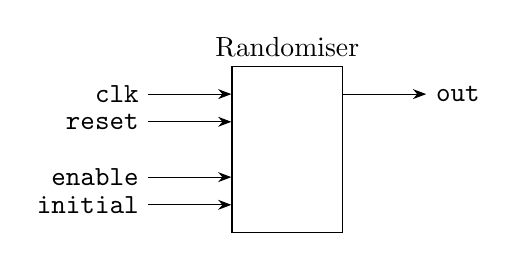
\begin{tikzpicture}
  [
    x=1em, y=1em,
    block/.style =
      {draw, rectangle, align=center, minimum width=4em, minimum height=6em},
    iarrow/.style =
      {<-, >={Stealth}, font=\ttfamily},
    oarrow/.style =
      {->, >={Stealth}, font=\ttfamily}
  ]

\node[block, label=above:Randomiser] (r) at (0,0) {};

\draw [iarrow] ($(r.west)+(0,2)$) -- ++(left:3) node[left] {clk};
\draw [iarrow] ($(r.west)+(0,1)$) -- ++(left:3) node[left] {reset};
\draw [iarrow] ($(r.west)-(0,1)$) -- ++(left:3) node[left] {enable};
\draw [iarrow] ($(r.west)-(0,2)$) -- ++(left:3) node[left] {initial};

\draw [oarrow] ($(r.east)+(0,2)$) -- ++(right:3) node[right] {out};

\end{tikzpicture}
  \caption{Randomiser Block Diagram}
  \label{RandomiserBlk}
\end{figure}

Implementing the randomiser is straight forward.
A possible set of taps for a 32-bit Galois LFSR is [32, 30, 26, 25].
Referring back at Figure~\ref{GalLFSR} on page~\pageref{GalLFSR},
the logic is to XOR the bits left of the taps with bit 0, and simple right shift for all other bits.
For driver to control the randomiser, an enable signal and an initial signal is added as input in addition to clock and reset.
The \texttt{initial} signal seeds the LFSR.

\section{Driver}

\begin{figure}[H]
  \centering
  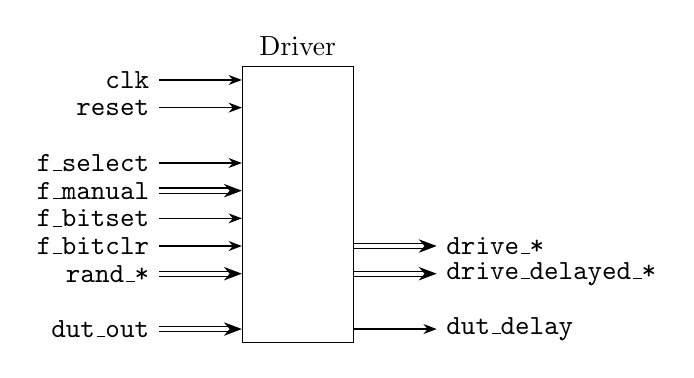
\begin{tikzpicture}
  [
    x=1em, y=1em,
    block/.style =
      {draw, rectangle, align=center, minimum width=4em, minimum height=10em},
    sarrow/.style =
      {>={Stealth}, font=\ttfamily},
    darrow/.style =
      {double distance=1.5pt, >={Stealth}, font=\ttfamily}
  ]

\node[block, label=above:Driver] (r) at (0,0) {};

\draw [<-, sarrow] ($(r.west)+(0,4.5)$) -- ++(left:3) node[left] {clk};
\draw [<-, sarrow] ($(r.west)+(0,3.5)$) -- ++(left:3) node[left] {reset};

\draw [<-, sarrow] ($(r.west)+(0,1.5)$) -- ++(left:3) node[left] {f\_select};
\draw [<-, darrow] ($(r.west)+(0,0.5)$) -- ++(left:3) node[left] {f\_manual};
\draw [<-, sarrow] ($(r.west)-(0,0.5)$) -- ++(left:3) node[left] {f\_bitset};
\draw [<-, sarrow] ($(r.west)-(0,1.5)$) -- ++(left:3) node[left] {f\_bitclr};
\draw [<-, darrow] ($(r.west)-(0,2.5)$) -- ++(left:3) node[left] {rand\_*};

\draw [<-, darrow] ($(r.west)-(0,4.5)$) -- ++(left:3) node[left] {dut\_out};

\draw [->, sarrow] ($(r.east)-(0,4.5)$) -- ++(right:3) node[right] {dut\_delay};

\draw [->, darrow] ($(r.east)-(0,1.5)$) -- ++(right:3) node[right] {drive\_*};
\draw [->, darrow] ($(r.east)-(0,2.5)$) -- ++(right:3) node[right] {drive\_delayed\_*};
\end{tikzpicture}
  \caption{Driver Block Diagram}
  \label{DriverBlk}
\end{figure}

The filter select signal \texttt{f\_select} selects the mode of operation of the driver.
When it is set, the driver will read from \texttt{f\_manual} and feed them to the output.
Otherwise, the driver will take the output of the randomisers at \texttt{rand\_*}, set and clearing specific bits according to \texttt{f\_bitset} and \texttt{f\_bitclr}.

The output is immediately sent to the DUT from the ports \texttt{drive\_dut\_*}.
The output is also delayed for a number of cycles before being sent to the monitor from the ports \texttt{drive\_mon\_*}.
This delay is known and thus can be configured by the user before compiling the testbench.

\begin{figure}[H]
  \centering
  \begin{tikztimingtable}
  [
    xscale=4,
    timing/d/background/.style={fill=white},
    timing/font=\ttfamily
  ]
  clk        & h 21{c} \\
  rand       & D{a4fe}D{527f}D{a93f}D{d49f}D{ea4f}D{7527}D{ba93}D{5d49}D{2ea4}D{1752}D{8ba9} \\
  f\_bitset  & 4D{0000} 7D{0004} \\
  f\_bitclr  & 3D{0000} 3D{f000} 5D{0000} \\
  drive\_dut & U D{a4fe}D{527f}D{a93f}D{049f}D{0a4f}D{0527}D{ba97}D{5d4d}D{1756}D{8bad} \\
  drive\_mon & 3U D{a4fe}D{527f}D{a93f}D{049f}D{0a4f}D{0527}D{ba97}D{5d4d} \\
  dut\_out   & 3U D{a4fe}D{527f}D{a93f}D{049f}D{0a4f}D{0527}D{ba97}D{5d4d} \\
\extracode
  % Add vertical lines in two colors
  \begin{pgfonlayer}{background}
    \begin{scope}[semitransparent,semithick]
      \vertlines{1,2,...,10}
    \end{scope}
  \end{pgfonlayer}
\end{tikztimingtable}
  \caption{Driver Waveform}
  \label{DriveWave}
\end{figure}

Figure \ref{DriveWave} shows how the waveform of the implemented driver looks like when operating in auto mode.
It should be stated that all waveforms in this report has been obtained from simulation, and are verified to be correct.
For clarity, unnecessary signals and signal values are omitted.

In the example waveform, we assume the design is a simple 1 input 1 output module where the input is passed to the output after 2 cycles.
The driver passed \texttt{rand} to \texttt{drive\_dut} after a cycle.
When \texttt{f\_bitclr} is \texttt{0xf000}, the top 4 bits of the output are set to 0, and when \texttt{f\_bitset} is \texttt{0x0004}, bit 2 of the output is set to 1.
It should be noted, that if the same bit is set and cleared by the user, \texttt{f\_bitclr} takes priority.
This is an arbitrary choice, and is noted in the user guide.

The driver delays the output to monitor by 2 cycles, and we can see that this aligns it the output from the DUT.

\section{Monitor}
\begin{figure}[H]
  \centering
  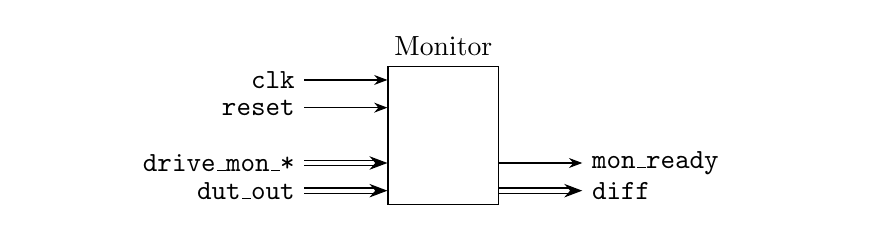
\begin{tikzpicture}
  [
    x=1em, y=1em,
    block/.style =
      {draw, rectangle, align=center, minimum width=4em, minimum height=5em},
    sarrow/.style =
      {>={Stealth}, font=\ttfamily},
    darrow/.style =
      {double distance=1.5pt, >={Stealth}, font=\ttfamily}
  ]

\node[block, label=above:Monitor] (r) at (0,0) {};
\node[draw, opacity=0, rectangle, minimum width=30em] () at (0,0) {};

\draw [<-, sarrow] ($(r.west)+(0,2)$) -- ++(left:3) node[left] {clk};
\draw [<-, sarrow] ($(r.west)+(0,1)$) -- ++(left:3) node[left] {reset};

\draw [<-, darrow] ($(r.west)-(0,1)$) -- ++(left:3) node[left] {drive\_mon\_*};
\draw [<-, darrow] ($(r.west)-(0,2)$) -- ++(left:3) node[left] {dut\_out};

\draw [->, sarrow] ($(r.east)-(0,1)$) -- ++(right:3) node[right] {mon\_ready};
\draw [->, darrow] ($(r.east)-(0,2)$) -- ++(right:3) node[right] {diff};

\end{tikzpicture}
  \caption{Monitor Block Diagram}
  \label{MonitorBlk}
\end{figure}

The monitor takes DUT inputs from the driver, and distributes them to a few sub-monitors.
Each sub-monitor containing a reference design then produces the correct results \texttt{mon\_out} from the inputs with a relaxed time budget.
The monitor then checks the difference between the reference output, \texttt{mon\_out}, and the DUT output, \texttt{dut\_out} with XOR gates.
This results in \texttt{diff}, where each bit set to 1 indicates a wrong bit in the DUT output.
\texttt{mon\_ready} will be set after the distributor has completed an entire round, where the first meaningful \texttt{diff} value becomes available.

As the number of sub-monitors and the width of the tested unit are parametrised, the design of the distributor was not straightforward.
An one-hot counter is set up to determined the currently active sub-monitor.
Since the sub-monitors are clocked \texttt{NUM\_SUB\_MON} times slower, an array of \texttt{NUM\_SUB\_MON} registers each of size \texttt{WIDTH} is also created for each input or output of the design.
These serves as the interface between the sub-monitors and the rest of the design.

\subsection{Sub-monitors}

\begin{figure}[H]
  \centering
  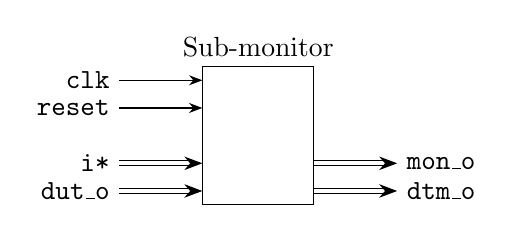
\begin{tikzpicture}
  [
    x=1em, y=1em,
    block/.style =
      {draw, rectangle, align=center, minimum width=4em, minimum height=5em},
    sarrow/.style =
      {>={Stealth}, font=\ttfamily},
    darrow/.style =
      {double distance=1.5pt, >={Stealth}, font=\ttfamily}
  ]

\node[block, label=above:Sub-monitor] (r) at (0,0) {};

\draw [<-, sarrow] ($(r.west)+(0,2)$) -- ++(left:3) node[left] {clk};
\draw [<-, sarrow] ($(r.west)+(0,1)$) -- ++(left:3) node[left] {reset};

\draw [<-, darrow] ($(r.west)-(0,1)$) -- ++(left:3) node[left] {i*};
\draw [<-, darrow] ($(r.west)-(0,2)$) -- ++(left:3) node[left] {dut\_o};

\draw [->, darrow] ($(r.east)-(0,1)$) -- ++(right:3) node[right] {mon\_o};
\draw [->, darrow] ($(r.east)-(0,2)$) -- ++(right:3) node[right] {dtm\_o};

\end{tikzpicture}
  \caption{Sub-monitor Block Diagram}
  \label{SubmonBlk}
\end{figure}

The current sub-monitor is a part of the monitor module in the architecture design that interfaces with the reference module.
In addition to connecting with the reference inputs and outputs, the sub-monitors also handles the delay of the reference module.
This is due to the highly parametrised nature of the monitor module, which made it rather complex and inflexible to the addition of more features.

As such, there is an extra signal of \texttt{dtm\_out}, which has the same value as \texttt{dut\_out}, but delayed by the number of cycles that the reference design needs to complete its operation, thus aligning with \texttt{mon\_out}.
The other signals are directly connected to the reference module.

\begin{figure}[H]
  \centering
  \begin{tikztimingtable}
  [
    xscale=4,
    timing/d/background/.style={fill=white},
    timing/font=\ttfamily
  ]
  clk           & h 19{c} \\
  dist\_ctr     & D{100} 3{D{001}D{010}D{100}} \\
  drive\_mon\_a & U D{0123} 2U D{3210} 2U D{0213} 2U \\
  drive\_mon\_b & U D{4567} 2U D{7654} 2U D{4657} 2U \\
  dut\_out      & U D{468a} 2U D{a861} 2U D{486a} 2U \\
  clk\_sub  [0] & 2L 2{2{c} 2L} 2{c} L \\
  a         [0] & 2U 3D{0123} 3D{3210} 2D{0213} \\
  b         [0] & 2U 3D{4567} 3D{7654} 2D{4657} \\
  dut\_o    [0] & 2U 3D{468a} 3D{a861} 2D{486a} \\
  mon\_o    [0] & 2U 3D{468a} 3D{a864} 2D{486a} \\
  diff          & 2U 3U D{0000} 2U D{0005} U \\
\extracode
  % Add vertical lines in two colors
  \begin{pgfonlayer}{background}
    \begin{scope}[semitransparent,semithick]
      \vertlines{1,2,...,9}
    \end{scope}
  \end{pgfonlayer}
\end{tikztimingtable}
  \caption{Monitor Waveform}
  \label{MonitorWave}
\end{figure}

Figure \ref{MonitorWave} shows the waveform of a monitor with \texttt{NUM\_SUB\_MON} as 3.
The reference adder takes 1 cycle to complete, but it must be clocked at a frequency slower than that of the adder DUT.
With 3 sub-monitors, the width of \texttt{dist\_ctr} is 3, and its lowest bit corresponds to sub-monitor 0, which is shown in detail in this figure.
\texttt{clk\_sub} is the clock driving the sub-monitor, which is made by masking the DUT clock with a delayed version of \texttt{dist\_ctr}.
As it ticks, the I/O values are copied into the register arrays and held for 3 cycles.
Within this time, the reference design completes its operation, fixing the value on \texttt{mon\_o}.
When the cycle of \texttt{dist\_ctr} goes a full cycle and the \texttt{sub\_clk} ticks again, this value is collected back and XOR'ed to form the final output of the monitor, \texttt{diff}.
In the example of Figure \ref{MonitorWave}, the second result was an error on the DUT, as it gave \texttt{0xa861} while the reference answer was \texttt{0xa864}.
This means bit 0 and 2 were different, and \texttt{diff} is thus \texttt{0x0005}.

The other sub-monitors all work identically but each 1 DUT cycle later the last.
This allows the reference design to run slower than the DUT, to still provide a constant stream of \texttt{diff} at the monitor output as designed.

\section{Scoreboard}

\begin{figure}[H]
  \centering
  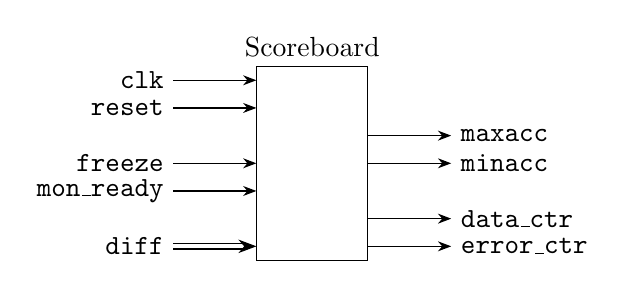
\begin{tikzpicture}
  [
    x=1em, y=1em,
    block/.style =
      {draw, rectangle, align=center, minimum width=4em, minimum height=7em},
    sarrow/.style =
      {>={Stealth}, font=\ttfamily},
    darrow/.style =
      {double distance=1.5pt, >={Stealth}, font=\ttfamily}
  ]

\node[block, label=above:Scoreboard] (r) at (0,0) {};

\draw [<-, sarrow] ($(r.west)+(0,3)$) -- ++(left:3) node[left] {clk};
\draw [<-, sarrow] ($(r.west)+(0,2)$) -- ++(left:3) node[left] {reset};

\draw [<-, sarrow] ($(r.west)+(0,0)$) -- ++(left:3) node[left] {freeze};
\draw [<-, sarrow] ($(r.west)-(0,1)$) -- ++(left:3) node[left] {mon\_ready};

\draw [<-, darrow] ($(r.west)-(0,3)$) -- ++(left:3) node[left] {diff};

\draw [->, sarrow] ($(r.east)+(0,1)$) -- ++(right:3) node[right] {maxacc};
\draw [->, sarrow] ($(r.east)+(0,0)$) -- ++(right:3) node[right] {minacc};

\draw [->, sarrow] ($(r.east)-(0,2)$) -- ++(right:3) node[right] {data\_ctr};
\draw [->, sarrow] ($(r.east)-(0,3)$) -- ++(right:3) node[right] {error\_ctr};

\end{tikzpicture}
  \caption{Scoreboard Block Diagram}
  \label{ScoreboardBlk}
\end{figure}

This scoreboard tracks the number of valid test points going through with \texttt{data\_ctr} and the number of errors within them with \texttt{error\_ctr}.
The external input \texttt{freeze} is exposed to the software to stop all counting in the scoreboard.
As the current HPS-FPGA bridge set up only allows sequential reads to the FPGA registers, it is necessary to ensure the values do not change within a single set of read commands from the software.

Another implication of the current bridge set up is that there is no simple way of getting all the \texttt{diff} values out to the HPS for statistics calculations.
This is a limitation of the current implementation, and will be discussed in the Further work section of this report.
Therefore, the hardware will have to do some simple statistics.

Since we are interested in how the precision of the DUT degrades as the frequency increases, two signals are created to record the maximum and the minimum precision of the DUT output.
Calculating the precision with the \texttt{diff} signal means counting the number of leading zeros (\texttt{CLZ}), as zeros indicate the correct bits.
As the current implementation is limited with a maximum width of 32, the easiest way of doing \texttt{CLZ} fast is by padding zeros after the number to 32 bits, and then use a large lookup table with don't cares.
This precision signal is named \texttt{acc}.

To keep track of the minimum precision, register \texttt{minacc} is first initialised to the maximum, and then for each smaller value observed, it will take on its smaller value.
The comparison logic here is relatively expensive in this fast testbench design.
As such, there is great incentive in the future to build a better communication method to allow offloading these operations to the HPS.

\begin{figure}[H]
  \centering
  \begin{tikztimingtable}
  [
    xscale=4,
    timing/d/background/.style={fill=white},
    timing/font=\ttfamily
  ]
  clk        & h 19{c} \\
  freeze     & 8L 2H \\
  mon\_ready & 2L 8H \\
  diff       & D{000f}D{0001}D{0000}D{0001}D{000c}2D{0000}3D{0001} \\
  data\_ctr  & 3D{0} 1R 6{Q} D{0} \\
  error\_ctr & 4D{0} D{1} 3D{2} D{3} D{4} \\
  maxacc     & 3D{0} 7D{16} \\
  minacc     & 3D{16} D{15} 6D{12} \\
\extracode
  % Add vertical lines in two colors
  \begin{pgfonlayer}{background}
    \begin{scope}[semitransparent,semithick]
      \vertlines{1,2,...,9}
    \end{scope}
  \end{pgfonlayer}
\end{tikztimingtable}
  \caption{Scoreboard Waveform}
  \label{ScoreboardWave}
\end{figure}

Figure \ref{ScoreboardWave} shows a example waveform.
The counters and the extrema trackers changes value only if we have \texttt{mon\_ready \&\& !freeze}.

\section{Wrappers}

Figure \ref{DBlock} provides a detailed look at how the individual hardware components are wired together to form the \texttt{testbench} module.
The DUT is shown as internal for clarity and it is the case during simulation testing of the testbench, but it should be understood that the DUT module is external in actual use.
The reference module similarly, is implied to be contained within the sub-monitor module, but this can be external during hardware use.

\begin{figure}[H]
  \centering
  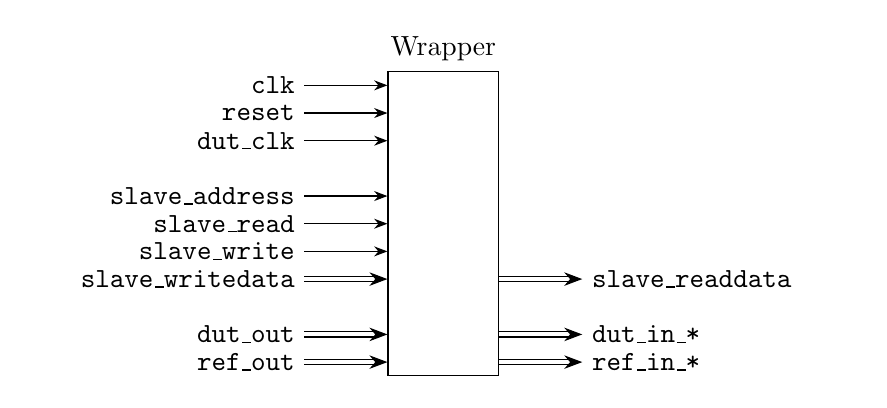
\begin{tikzpicture}
  [
    x=1em, y=1em,
    block/.style =
      {draw, rectangle, align=center, minimum width=4em, minimum height=11em},
    sarrow/.style =
      {>={Stealth}, font=\ttfamily},
    darrow/.style =
      {double distance=1.5pt, >={Stealth}, font=\ttfamily}
  ]

\node[block, label=above:Wrapper] (r) at (0,0) {};
\node[draw, opacity=0, rectangle, minimum width=30em] () at (0,0) {};

\draw [<-, sarrow] ($(r.west)+(0,5)$) -- ++(left:3) node[left] {clk};
\draw [<-, sarrow] ($(r.west)+(0,4)$) -- ++(left:3) node[left] {reset};
\draw [<-, sarrow] ($(r.west)+(0,3)$) -- ++(left:3) node[left] {dut\_clk};

\draw [<-, sarrow] ($(r.west)+(0,1)$) -- ++(left:3) node[left] {slave\_address};
\draw [<-, sarrow] ($(r.west)+(0,0)$) -- ++(left:3) node[left] {slave\_read};
\draw [<-, sarrow] ($(r.west)-(0,1)$) -- ++(left:3) node[left] {slave\_write};
\draw [<-, darrow] ($(r.west)-(0,2)$) -- ++(left:3) node[left] {slave\_writedata};

\draw [<-, darrow] ($(r.west)-(0,4)$) -- ++(left:3) node[left] {dut\_out};
\draw [<-, darrow] ($(r.west)-(0,5)$) -- ++(left:3) node[left] {ref\_out};

\draw [->, darrow] ($(r.east)-(0,2)$) -- ++(right:3) node[right] {slave\_readdata};

\draw [->, darrow] ($(r.east)-(0,4)$) -- ++(right:3) node[right] {dut\_in\_*};
\draw [->, darrow] ($(r.east)-(0,5)$) -- ++(right:3) node[right] {ref\_in\_*};

\end{tikzpicture}
  \caption{Test Wrapper Block Diagram}
  \label{WrapperBlk}
\end{figure}

\begin{sidewaysfigure}
  \begin{figure}[H]
    \centering
    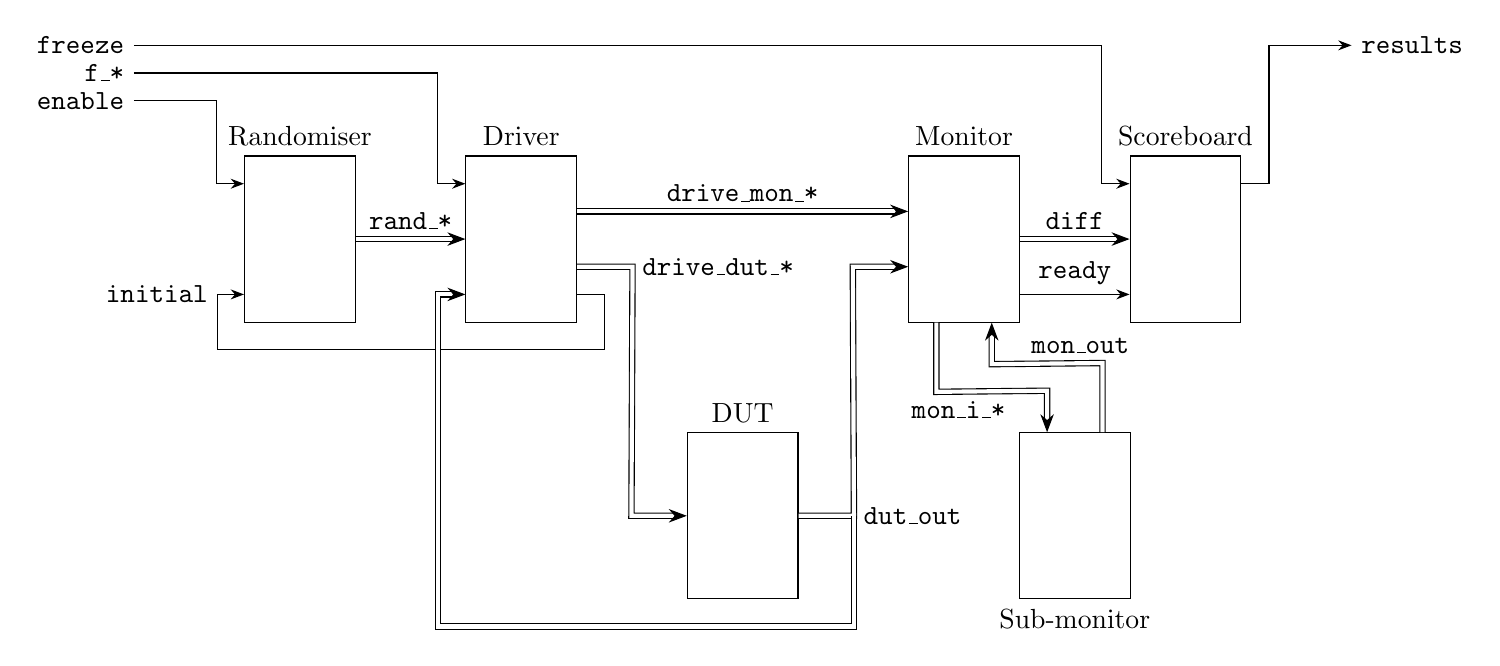
\begin{tikzpicture}
  [
    x=1em, y=1em,
    block/.style =
      {draw, rectangle, align=center, minimum width=4em, minimum height=6em},
    sarrow/.style =
      {>={Stealth}, font=\ttfamily},
    darrow/.style =
      {double distance=1.5pt, >={Stealth}, font=\ttfamily}
  ]
  \node [block, label=above:Randomiser]  at ( 8, 10)  (r) {};
  \node [block, label=above:Driver]      at (16, 10)  (d) {};
  \node [block, label=above:DUT]         at (24,  0)  (t) {};
  \node [block, label=above:Monitor]     at (32, 10)  (m) {};
  \node [block, label=below:Sub-monitor] at (36,  0)  (u) {};
  \node [block, label=above:Scoreboard]  at (40, 10)  (s) {};

  \draw [->, sarrow] (2,15) node[left] {enable}
                      -| ($(r.west)+(-1,2)$)
                      -- ($(r.west)+(0,2)$);
  \draw [->, sarrow] (2,16) node[left] {f\_*}
                      -| ($(d.west)+(-1,2)$)
                      -- ($(d.west)+(0,2)$);
  \draw [->, sarrow] (2,17) node[left] {freeze}
                      -| ($(s.west)+(-1,2)$)
                      -- ($(s.west)+(0,2)$);

  \draw [->, sarrow] ($(d.east)-(0,2)$)
                      -| ++(1,-2)
                      -- ++(-14,0)
                      |- node[left] {initial} ($(r.west)-(0,2)$);
  \draw [->, darrow] ($(r.east)+(0,0)$)
                      -- node[above] {rand\_*} ($(d.west)+(0,0)$);
  \draw [->, darrow] ($(d.east)+(0,1)$)
                      -- node[above] {drive\_mon\_*} ($(m.west)+(0,1)$);
  \draw [->, darrow] ($(d.east)-(0,1)$)
                      -- ++(2,0)
                      -- node[right,pos=0] {drive\_dut\_*} ($(t.west)+(-2,0)$)
                      -- ($(t.west)+(0,0)$);
  \draw [->, darrow] ($(t.east)-(0,0)$)
                      -- ++(2,0)
                      -- node[right,pos=0] {dut\_out} ($(m.west)-(2,1)$)
                      -- ($(m.west)-(0,1)$);
  \draw [->, darrow] ($(t.east)+(2,0)$)
                      |- ($(d.west)-(1,14)$)
                      |- ($(d.west)-(0,2)$);
  \draw [->, darrow] ($(m.south)-(1,0)$)
                      -- ++(0,-2.5)
                      -- node[below,pos=0.2] {mon\_i\_*} ($(u.north)-(1,-1.5)$)
                      -- ($(u.north)-(1,0)$);
  \draw [<-, darrow] ($(m.south)+(1,0)$)
                      -- ++(0,-1.5)
                      -- node[above,pos=0.8] {mon\_out} ($(u.north)+(1,2.5)$)
                      -- ($(u.north)+(1,0)$);
  \draw [->, darrow] ($(m.east)+(0,0)$)
                      -- node[above] {diff} ($(s.west)+(0,0)$);
  \draw [->, sarrow] ($(m.east)-(0,2)$)
                      -- node[above] {ready} ($(s.west)-(0,2)$);
  \draw [->, sarrow] ($(s.east)+(0,2)$)
                      -| ++(1,5)
                      -- (46,17) node[right] {results};

\end{tikzpicture}
    \caption{Block diagram of the implemented testbench}
    \label{DBlock}
  \end{figure}
\end{sidewaysfigure}

The inputs and outputs of this module is contained within \texttt{test\_wrapper}, which handles the AXI communications when coupled with the \texttt{hps} module.
This allowed the software to access the testbench, completing the overall system implementation.
In addition to the AXI interface, the conduits to external design and reference modules, we should also see that the wrapper has two clock inputs, since the AXI interface is clocked differently to the rest of the testbench.

All I/O signals are given an address on the HPS-FPGA Bridge.
They are listed as follows in Table \ref{MemLoc}.
The prefix \texttt{I}, \texttt{O}, or \texttt{D} indicates that the register is write only, read only, or read/write respectively.
All register names follow closely to that of the signal, except for \texttt{reset}, \texttt{enable}, and \texttt{freeze}, which has been collected into one \texttt{D\_CTRL} register.
They are bit 0, 1, and 2 of the register, respectively.

\begin{table}[H]
  \centering
  \begin{tabular}{|>{\ttfamily}l|>{\ttfamily}l|}
    \hline
    \textrm{Register}   & \textrm{Location} \\
    \hline
    D\_CTRL       & 6'h00 \\
    O\_SYSVER     & 6'h04 \\
    \hline
    I\_FSELECT    & 6'h10 \\
    I\_FMANUAL\_A & 6'h14 \\
    I\_FMANUAL\_B & 6'h18 \\
    I\_FBITSET\_A & 6'h1C \\
    I\_FBITSET\_B & 6'h20 \\
    I\_FBITCLR\_A & 6'h24 \\
    I\_FBITCLR\_B & 6'h28 \\
    O\_DUTDELAY   & 6'h2C \\
    \hline
    O\_DATCTR     & 6'h30 \\
    O\_ERRCTR     & 6'h34 \\
    O\_MAXACC     & 6'h38 \\
    O\_MINACC     & 6'h3C \\
    \hline
  \end{tabular}
  \caption{Memory Locations in the Test Wrapper}
  \label{MemLoc}
\end{table}

The listed values are relative addresses.
As specified in the manual, the lightweight bridge is physically at \texttt{0xFF20\_0000}~\cite{Altera6}.
As the golden reference design already uses some of the lower values in this bridge, an offset address of \texttt{0x0010\_0000} was given to the test wrapper.
For example, the physical address of \texttt{O\_SYSVER} is \texttt{0xFF30\_0004}.
The PLL configuration also shares the same bridge, so it was given an offset address of \texttt{0x0011\_0000}.


\chapter{Software Implementation}

\section{Accessing the FPGA}
The interfaces are mapped onto the physical memory, thus they can be accessed by opening \texttt{/dev/mem} with the \texttt{mmap} library in the Python test script.
The 4 bytes of binary data from the FPGA also needs to be packed or unpacked with the \texttt{struct} library, as they needs to be interpreted as unsigned long integers in little-endian.
The read and write function are defined in a class called \texttt{axi}.
The base of this function is provided to me by my supervisor.

Since the design is to abstract away direct interactions with the memory locations in the test wrapper, another class called the \texttt{wrapper} is created to serve as a collection of useful read and write functions.
Similarly, a class called \texttt{pll} is created to serve the same purpose, but for the PLL reconfiguration module.
The initial version of the \texttt{pll} class was provided to me by my supervisor, but it was then modified to provide more flexibility in frequency control.

A brief summary of the PLL configuration is as follows.
There are 3 reconfigurable stages from the input frequency $f_{in}$ to the output frequency $f_{out}$, called $M$, $N$, and $C$.
$M$ is a multiplier, and $N$, and $C$ are dividers, or in an equation,
$f_{out} = f_{in} \times \frac{M}{N \times C}$.
Each stage can be individually bypassed, and there can be multiple parallel $C$ stages in a single PLL to provide multiple frequencies outputs.

Converting from the desired divisor or multiplier to binary write data is not trivial, but it can be written into a function as all the rules are stated in the user manual~\cite{Altera7}.
After writing it in, the software waits for the hardware to finish configuring by watching another memory location, and then returns the frequency set.
This may deviate from the desired frequency due to hardware limitations of the PLL.

To illustrate the abstraction, we can examine what happens when the user writes the command \texttt{reset} to reset the entire system.

First the software calls the \texttt{cleanreset} function in class \texttt{wrapper}.
This calls the a function to set the reset bit and then clears it.
It also clears the enable signal and the freeze signal.
Then it writes all zeros to all driver filter control registers, completing the wrapper side reset.
Then the software calls a function in class \texttt{pll}, which sets the PLL frequency back to the default value, thus fully resets the whole system.

\section{Read-eval-print Loop}

To set up a REPL, a list of expressions that the user is allowed to give to the program is defined as in Table \ref{REPL Commands}.
These commands are made to be intuitive to the user, yet retaining all functional control of the system.

\begin{table}[H]
  \centering
  \begin{tabular}{|>{\ttfamily}p{11em}|p{\dimexpr\textwidth-18em}|}
    \hline
    \textrm{Command}   & Explanation \\
    \hline
    reset              & Resets the system and test results. \\
    version            & Prints the system version. \\
    freq <speed>       & Sets the clock speed to the specified value in MHz. Prints the actual frequency configured. \\
    mode <m|a>         & Choose between \underline{m}anual and \underline{a}uto test mode. \\
    manual <a|b> <hex> & Give input in manual mode. \\
    bitset <a|b> <hex> & Force bits to be 1 in auto mode. \\
    bitclr <a|b> <hex> & Force bits to be 0 in auto mode. \\
    run <time>         & Runs the test for specified duration in ms. Prints the results at the end of the test. \\
    exit               & Exits the REPL. \\
    \hline
  \end{tabular}
  \caption{Commands accepted in test REPL}
  \label{REPL Commands}
\end{table}

As user friendliness is a major concern in this project, the user inputs are not assumed to be always syntactically correct.
Therefore, the raw inputs are first sent through a series of checks to make sure they are valid.
This means the command must be in the list, they must be supplied with the correct number of arguments, and all arguments are in a valid form.
If any of the tests failed, the command will not ran and a helpful error message will be printed.
Otherwise, the command will be passed with a parser and translated to read and write instructions to the FPGA.

A debug feature is also provided in the software, so the user can choose to run the program in a sandbox first before running it on actual hardware.
This is done with the built-in constant \texttt{\_\_debug\_\_} in Python.
If the user decides to run the script in debug mode with \texttt{python ./run\_test.py}, the script will not actually write or read anything in the FPGA, but print out the address of all locations that it will be writing or reading in a real run.
To actually run the test, the user should use \texttt{python -O ./run\_test.py} to disable debug mode.

\section{Automation}

The initial disadvantage of a REPL program is that it requires inputs from the users every time they wishes to do something.
This can quickly get tedious, so to counter this issue, we have set up an automation system.
Now the users can write all the commands that they wants to run into a file, and the script will parse them the same as in REPL mode line-by-line.

This is implemented with a check for \texttt{argv} after the program starts.
If there is an argument provided when the program is called, as in \texttt{python -O ./run\_test.py test.do}, then the program will jump to the automated mode, and if there is no arguments, the program will start in REPL mode.
This syntax should be familiar to users, as this is how the \texttt{python} command and many other command line program works.


\chapter{System Integration}

\section{Qsys}


\newpage
\chapter{Out-of-the-box Testing}

\section{Introduction}
In an out-of-the-box test, the product is delivered to test users as a packaged box.
Then the unpacking process, in which the users sets up and uses the product, is observed to study the intuitiveness of the design.
This testing method is used in this project as one of the key determinant for the success of this project is how convenient it is for users to configure and make use of the framework.

For this project, we have made up a scenario where the users have designed an adder with a suspected error that they wish to ascertain.
The user guide [Appendix \ref{appendix:guide}], the testbench, and a flawed adder design was provided to the test volunteers.
If both inputs to the adder are o
The test volunteers were made aware that there might be error is


\section{Results}
% REVISIT: What to put here?

\chapter{Evaluation}

\section{Product Metrics}
\subsection{Robustness}
As planned in the interim report, we will use 3 metrics to evaluate the performance of the final product.
First, the maximum stress of which the testbench can provide without failing is a good metric.
This can be quantitatively measured by the maximum data throughput across the DUT, and the maximum frequency that the DUT can be running where the testbench remains reliable.
A robust testbench with a higher maximum frequency can reveal a wider picture in the performance of the DUT.
This would hopefully allow more insights to be gained regarding the DUT, or it could mean that the testbench can be used for future designs that may be faster than the current one.

To measure this, we can run \textit{TimeQuest} on the compiled design to obtain software estimations of the speed of the design.
The worst case scenario is a 1100mV model running at 85$^\circ$C.
Under this condition, the restricted $f_{max}$ is reported as 394.01MHz.
However, software estimations are usually conservative, so hardware tests were run to complement the results.
After compiling the design on to a FPGA, it was observed that the test was reasonably stable at 400MHz, but breaks frequently at 425MHz.

Although this did not reach the initial goal of 600MHz set in the design phase of the project, it is still high enough to be capable of testing a wide range of designs.
This number can be further optimised by pipelining the slowest signal paths and reducing the latency in each cycle.
The initial $f_{max}$ estimation before the frequency optimisation was at 210MHz.
Because it is a relatively time consuming task with diminishing returns, and does not provide any functional improvement to the implementation, it was dropped for more important work once the milestone of 400MHz was reached.

Overall this is still a satisfactory result, as the frequency still comfortably higher than that of the arithmetic unit, which was assumed to run at 300MHz.
Just to compare the hardware acceleration, we timed a software simulation of the same testbench.
It managed to process 42000 data points in a second, which is equivalent to 42kHz, making the FPGA roughly 10000 times faster than software.

\subsection{Flexibility}
As the framework is designed to be extensible and widely applicable, the flexibility of the testbench is also vital to the product's performance.
This can be measured by the number of configurable parameters that it has, and the range of which these parameters can be adjusted to.

\begin{table}[H]
  \centering
  \begin{tabular}{|l|c|p{15em}|}
    \hline
    Item                  & Reconfigurability & Explanation \\
    \hline
    \texttt{WIDTH}        & $\le$32 bits & Design I/O width \\
    \texttt{NUM\_SUB\_MON}& $\ge$2       & Varies time constraint ratio between DUT and reference \\
    $f_{\text{dut}}$             & $\le$400MHz  & Frequency of the DUT \\
    bitset/bitclr         & All values & Forces bits in test data in auto mode \\
    manual                & All values & Sets test data in manual mode \\
    time                  & All values & Sets test duration \\
    design I/O            & 2 in 1 out & Number of inputs and outputs supported for design \\
    \hline
  \end{tabular}
  \caption{Configurable and Fixed Options}
  \label{ProdOpt}
\end{table}

Most of these items have been discussed in detail in the previous chapters.
The entry on test duration shows that the test data generation and transfer system design removes the upper limit in how long the test can continuously run.
This is useful if the user is interested in stressing the FPGA at a high temperature.

While the testbench implementation already allows for a great variety of DUTs to be tested, there are still featural limitations that may become deal breakers for some users.
\begin{enumerate}
  \setlength\itemsep{0pt}
  \item The driver filtering in auto mode is limited to bit-wise manipulation.
  \item The DUT can only have 1 or 2 inputs and 1 output.
  \item The FPGA has no way of transferring all \texttt{diff} data out to the HPS at-speed.
  \item The testbench was built with a 32 bits maximum width in mind.
        This is reflected on how the LFSRs in the randomiser have 32 bits, and how the \texttt{CLZ} operation in scoreboard is implemented with a lookup table.
\end{enumerate}

Looking at the lists, we can conclude that the product is reasonably flexible, but more importantly, as a prototype, the implementation has demonstrated the flexibility and the extensibility of the framework design.
How we might loosen these limitations and exploit more of the potential from the framework design will be discussed in the Further Work section of this report.

\subsection{User-friendliness}
The ease of use of the testbench can be another evaluation point.
Having a plethora of knobs and switches makes a powerful testbench, but no one would want to use the testbench if the effort to understand and start working with it is overwhelming.
As such the framework also needs to be critiqued for its user-friendliness.

The product has been designed and built with the users in mind every step of the way, and the usability has been studied with the OOTB test in the Testing chapter.
In hardware, we have exposed the DUT and the reference conduits from the test wrapper to allow easy swapping of different test designs with Qsys.
All configurable parameters are made editable from the same interface of Qsys.
In software, the REPL is built so that the users can interact intuitively with the FPGA.
We have also created a debug mode for the users since we understand that debugging hardware can be a convoluted process, and presenting insightful information to the users can be greatly beneficial.

From the design perspective, the framework is modular with each module having one obvious main purpose.
This means the expert users can easily modify the implementation if additional functionalities are desired.
This is the same for both hardware and software.

Nevertheless, the product still has potential to serve the users better.
The users are still required to use Qsys and Quartus to enter a few parameters and make a few connections before compiling the hardware.
They are then tasked to upload the test software and program the FPGA, before being able to start running tests with the REPL or macro files.
In all, they have to perform inputs in 4 different locations, and as shown during the OOTB test, if a mistake made early in the process may not surface until the very end.

\section{Project Metrics}
Aside from evaluating the product itself, we should also have a brief analysis at the project level.
We first examine at the project plan proposed in the interim report.
8 tasks were laid out onto a timeline in section 5.1.
2 were already complete by the submission of interim report, leaving 3 core tasks and 3 extension tasks to do until the submission of this report.
The 3 core tasks were done on time, but there was a major delay during the first extension task, which was titled \textit{Configurable Modules}.
Instead of taking one and a half weeks as planned, it took more than a month to complete.
The details and the resolution of the problem were discussed in section 10.1.2 and 10.1.2.

Since we have planned in slacks for each task, this delay did not hit the project as hard as it could have without.
The next task of \textit{Handling Failures} was cut short, so while the basics features such as providing accuracies of failed outputs and statistical data was built, the added reconfigurability for the verbosity of the statistics was not made available so the output of the testbench is always the same.
The initial reasoning for providing varying verbosity was that we were worried that additional logic would slow down the system, so the user will have the choice between having faster tests or having more detailed results.
As we have limited the maximum width of the implementation at 32, the additional logic was built with lookup tables and other components that did not slow down the system as much.
The final task of \textit{Interactive UI} was fully complete as an interactive command line interface was built.
In addition, it also had automation capabilities with macro files, which was a feature beyond what was planned for this task in the previous report.

As stated in the interim report section 6.2.2, there will always be more potential for further work.
The list of limitations and potential improvements of the product was thus within expectation, and should not be considered as a failure on the project level.
Therefore, we can claim that the project was reasonably successful on both the management and the execution level.


\section{Conclusion}

\section{Further Work}

\section{User Guide}

\newpage
%\setstretch{1.0}
\appendix
\chapter{User Guide Provided to Test Volunteers}

\chapter{Raw Data}

\textcolor{red}{+Code Snippets?}


\newpage
\input{tex/bibliography}

\end{document}